\chapter[Under pressure, ICP in Traumatic Brain Injury]{Under pressure, ICP in Traumatic Brain Injury}
Intracranial pressure (ICP) is a critical parameter in the management of traumatic brain injury (TBI), serving as a window into the brain’s dynamic response to injury. After a traumatic event, the brain’s natural mechanisms to regulate pressure — via fluid shifts, blood flow adjustments and tissue compliance as according to Monro-Kellie doctrin — are often compromised. \\

Elevated ICP is one of the most determinant complications in TBI, as it not only reflects underlying pathology but also drives secondary brain injury by reducing cerebral perfusion, increasing ischemia, and damaging neuronal tissue. Even small shifts in intracranial dynamics can dictate life-or-death outcomes, making ICP not only a marker of injury but also a factor in the recovery process.

In brain-injured adults, an intracranial pressure (ICP) greater than 20-22 mmHg is generally recognised as the threshold for intracranial hypertension\cite{hawrylukIntracranialPressureCurrent2022a}. However, while this is important, the interpretation of ICP is far more complex than the value itself\cite{cuccioliniIntracranialPressureClinicians2023a}.\\

\section[Brain volumes, intracranial components]{Brain volumes, intracranial components}
It was all the way back to the 1783 when Monro stated that the blood contenent within the skull should have been constant, so the amount of inflow should have equalized the outflow. Kellie perfectioned this assumption: any volume within the skull cannot be displaced without being replaced by another component, when a displacement is not possible a consequent increase in intracranial volume would result in increased ICP.\\

While often described as static component as it is nearly incrompressible, the brain parenchyma (the functional tissue of the brain) can actually change its volume over time, shrinking in response to injury or swelling, primarily in the component of glial cells. This tissue modification occurs gradually, impacting the brain's compliance (its ability to tolerate changes in volume without relevant changes in brain pressure).\\

The blood volume instead, both in the arterial and venous compartment, significantly influence ICP. 

The arterial side can rapidly adjust cerebral blood flow (CBF) by constricting or dilating blood vessels within seconds. The so-called \textit{cerebral autoregulation} keeps the CBF constant despite fluctuations in systemic blood pressure. This ennsures that the brain receives a consistent supply of oxygen and nutrients, even when blood pressure changes. Cerebral autoregulation operates effectively within a specific range of mean arterial pressure (MAP), typically between 60 and 150 mmHg in healthy individuals. New insights would otherwise suggest though a more narrow range as smaller pial arteries dilates more than bigger arteries, consequently important intersubject variability for active autoregulation does exist\cite{kleinDifferentialHemodynamicResponse2022}. 

The venous compartment plays a crucial role in ICP determination. Nearly 70\% of blood makes up a significant portion of the total blood in the brain is venous within the skull, CVP is then closely linked to ICP. Bridging veins form a connection between the brain’s deep venous and superficial venous systems. Closely associated with cerebrospinal fluid, these veins consist primarily of intima tissue, making them highly collapsible and distensible. As a result, they function like a Starling resistor, preventing retrograde transmission of abrupt increase of central venous pressure (CVP) to ICP. However, as ICP increases, the bridging veins begin to collapse, raising outflow resistance. Once a critical closing pressure is reached, venous outflow is halted entirely\cite{wilsonMonroKellie20Dynamic2016}.\\

Cerebrospinal fluid (CSF), though relatively small in volume compared to other components (about 150ml), is vital for maintaining pressure equilibrium within the skull, distributing and equalising changes in ICP. The concept of \textit{CSF compensatory reserve}, which refers to the CSF’s ability to accommodate volume fluctuations without altering intracranial pressure (ICP), depends on the lumbar sac’s capacity for expansion and the continuous fluid exchange within the recently explored glymphatic system\cite{cuccioliniIntracranialPressureClinicians2023a}.\\

Each cerebral volume exhibits its own dynamic and contributes to compensate for any rise in ICP, through various chemical and physical mechanisms and at different rates. The ICP reflects the overall system’s elasticity and compliance.\\

\section[Cerebral compliance, the silent buffer]{Cerebral compliance, the silent buffer}
The relationship between pressure and volume defines the compliance of a system, so one does exists also for the brain and express the relationship between any increase in volume related to an increase in ICP.

At first, volume increases cause only a slight rise in pressure so long as the compensation systems and cerebral autoregu- lation work, but once the system’s buffering capacity is exceeded, ICP rises steeply.
These changes are not necessarily associated with specific ICP number thresholds, as we can find patients with signs of intracranial hypertension within a “normal range” of ICP as patients that still demonstrate a good compliance in spite of ICP above thresholds (see fig.2.2). \\

\begin{figure}[h]
    \centering
    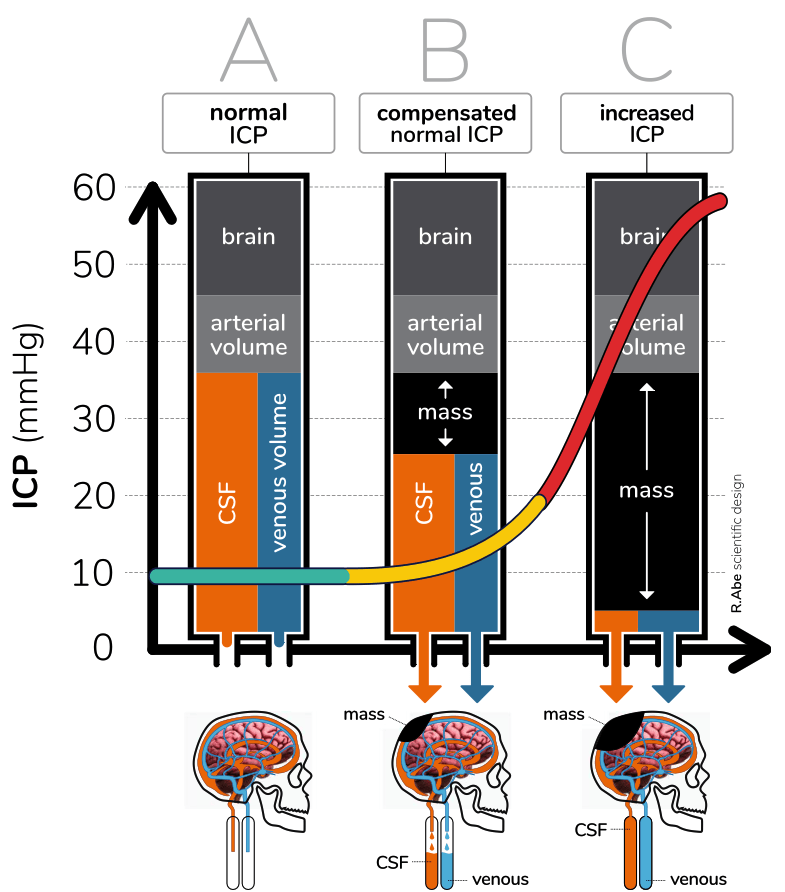
\includegraphics[width=0.6\textwidth]{pictures/fig2.png}
    \caption{Different phases of the cerebral compliance. In the first phase (A), compensatory system is effective and ICP does not change. In a second phase (B), the compensatory system starts to fail following more increase in volume. CSF and veins outflow are starting to be overloaded, beginning brain deformation and CBF impairment. In a third phase (C), the compensatory system is exhausted, brain deformation and loss of compliance are evident. Modified from Godoy et al.\cite{godoyIntracranialCompartmentalSyndrome2023a}}
\end{figure}

Following traumatic brain injury, both intracranial and systemic factors contribute to the rise in intracranial pressure. In the initial hours after injury, expanding hematomas pose the greatest risk. However, in the days that follow, other mechanisms such as fluid accumulation, impaired autoregulation, ischemia, and the expansion of contusions further increase intracranial pressure. When a mass lesion forms, it creates a pressure gradient that distorts brain tissue, leading to midline shifts and brain displacement either medially or caudally, resulting in herniation, a medical emergency that requires immediate intervention to prevent irreversible and often fatal damage to the brainstem.

The vascular consequences of elevated intracranial pressure arise from reduced cerebral perfusion pressure (CPP, as the difference between mean arterial pressure and intracranial pressure). CPP drives cerebral blood flow but the adequate one vary between patients. As CPP declines, cerebral blood flow may become insufficient for proper tissue perfusion, leading to ischemia. This, in turn, triggers cytotoxic edema, exacerbating intracranial pressure even further\cite{stocchettiTraumaticIntracranialHypertension2014a}.\\

\section[ICP waveform, more than a number]{ICP waveform, more than a number}
The intracranial pressure (ICP) waveform is a graphical representation of pressure changes within the skull over time. It reflects the pulsatile nature of ICP, influenced by arterial blood flow, venous outflow, and cerebrospinal fluid (CSF) dynamics.
The classical representation of the waveform is the one we see at the bedside that shows ICP over time (time domain representation)\footnote {The frequency domain representation also exists, but it requires additional software and hardware for the spectral anaylisis \cite{cuccioliniIntracranialPressureClinicians2023a}}.\\
The ICP waveform in the time domain can provide different insights depending on the duration being analyzed, ranging from moments or seconds to a timeframe as long as one hour.

The waveform is typically divided into three main components or peaks:
\begin{enumerate}
    \item \textbf{P1 (Percussion wave)}: This represents the arterial pressure transmitted through cerebral arteries, synchronous with the systolic peak of the arterial waveform.
    \item \textbf{P2 (Tidal wave)}: the second peak is directly proportional to the brain’s compliance as it represent the increase in cerebral blood volume. In a normal ICP waveform, P2 is lower than P1, indicating good cerebral compliance. When P2 is higher than P1, it suggests reduced compliance, meaning the brain’s ability to compensate for volume changes (like increased blood volume or swelling) is diminished.
    \item \textbf{P3 (Dicrotic wave)}: Corresponds to the closure of the aortic valve and reflects venous outflow. It is typically the smallest of the three peaks.
\end{enumerate}
In healthy individuals or patients with good cerebral compliance, the waveform shows a descending pattern where P1 > P2 > P3. As brain compliance decreases, P2 rises and surpasses P1. In the final more severe stage, the waveform resemble a triangular shape, where the individual peaks are no longer distinguishable.
The \textit {P1/P2 ratio} reflects this relationship, reflects this relationship, with a normal ratio being greater than 1. In pathological conditions, values of 1 or less are typically observed.\\

Zooming out on the timeline new waveforms pattern can arise. Those are called \textit{Lundberg waves} and are classified as: 
\begin{itemize}
    \item \textbf{A waves or “plateau waves”:}
    These are characterized by a rise in ICP until a plateau phase followed by a decrease, often reaching values of 50-100 mmHg, lasting for several minutes (5-20 minutes).
    They are consequence of a drop in arterial blood pressure (ABP) that causes cerebral vasodilation, reducing cerebral perfusion pressure (CPP), leading to more vasodilation and higher ICP. As plateau waves represent a temporary brain hypoperfusion, those are often associated with ischemia and prompt intervention to prevent irreversible brain damage is needed. To note, plateau waves can also terminate spontaneously after a few minutes. Are associated with critically reduced cerebral compliance, tipically found in young patients with low midline-shift.

    \item \textbf{B waves:} B waves are oscillations in ICP within 10 to 20 mmHg. They last 30s to a couple of minutes and are often associated with increase in CBF so are related to  brain metabolism. They're meaning is contradictory: fore some  are early indicators of impaired  compliance, for others the greater the amplitude of B waves the better is the outcome\cite{cuccioliniIntracranialPressureClinicians2023a}.
 
    \item \textbf{C waves:} C waves are the least significant clinically, often linked to autonomic nervous system activity. 
  
    \item \textbf{Respiratory waves}: Respiratory waves are synchronous with breathing, they've been associated with increased resistance to CSF circulation so can correlate with intracranial compliance in patients with hydrocephalus.\\

\end{itemize}

\begin{figure}[h]
    \centering
    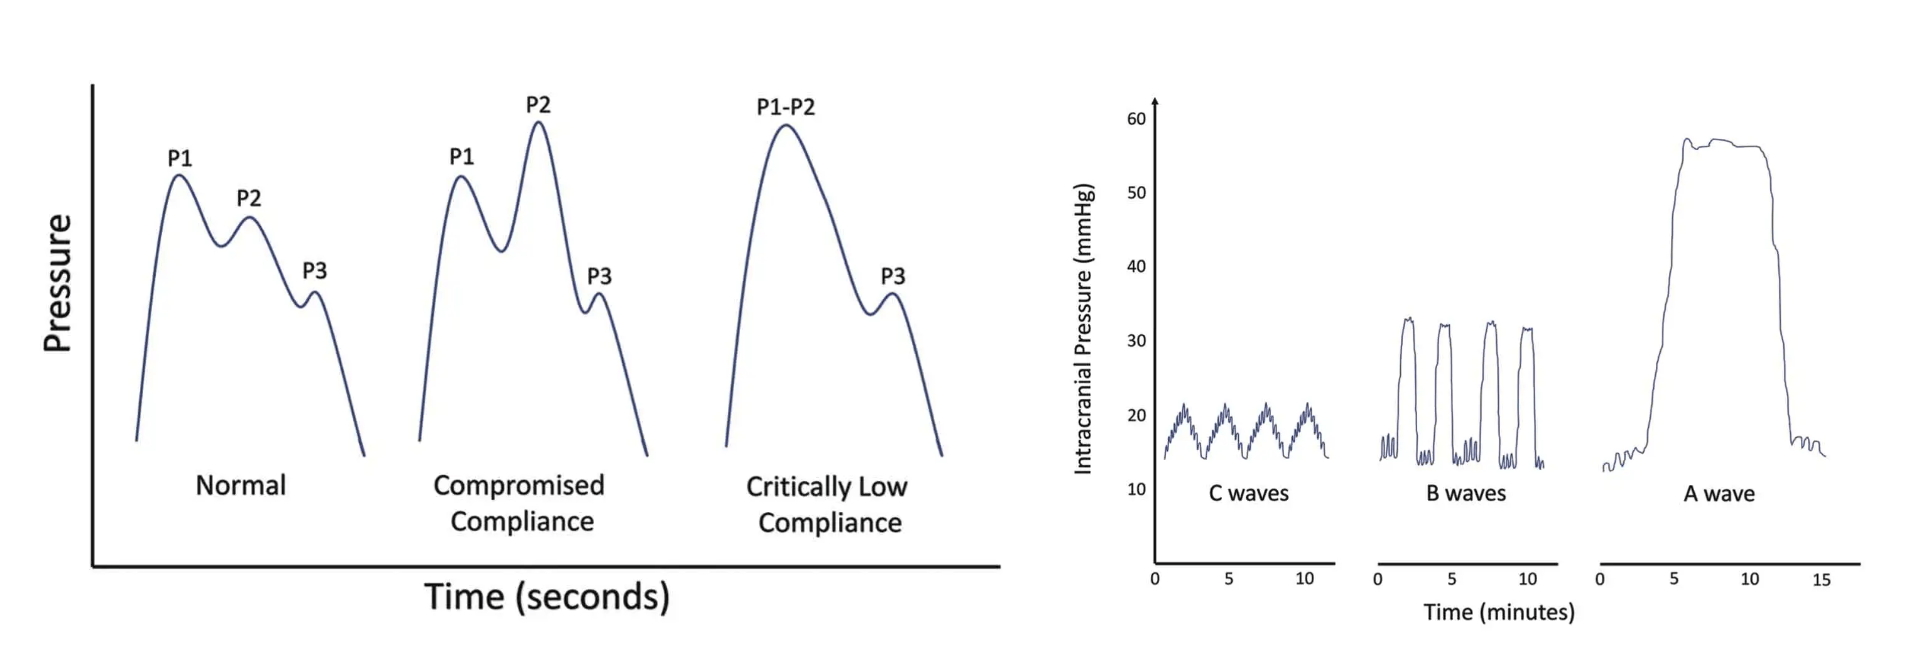
\includegraphics[width=0.8\textwidth]{pictures/fig3.png}
    \caption{Left: Intracranial pressure (ICP) waveforms. Normal waveform shows P1>P2>P3, with compromised intracranial compliance P2>P1. \\ Right: Lundberg intracranial pressure waves. A waves reflect critically exhausted intracranial compliance. B waves likely occur because of impaired cerebral perfusion and may suggest impaired intracranial compliance. C waves may be seen in normal physiology and are likely related to sympathetic activity. Modified from Liotta et al.\cite{liottaManagementCerebralEdema2021}}
\end{figure}

\section[The pressure within, ICP monitoring]{The pressure within, ICP monitoring}
All international guidelines provide the ICP threashold of 22mmHg as the cutoff to start treatment. But to know this value we have to monitor ICP in the first place.\\

 Intracranial pressure monitoring is recommended for all patients with survivable severe traumatic brain injury who show abnormalities on the admission computed tomography (CT) scan. Additionally, monitoring is advised for certain patients with a normal CT scan, such as those over 40 years of age with hypotension or abnormal pain responses (e.g., abnormal flexion or extension).
An external ventricular drain (EVD) is placed in a brain ventricle and connected to a transducer for monitoring intracranial pressure (ICP). While alternative invasive methods, such as intraparenchymal probes, microstrain gauges, and fiberoptic catheters, are gaining popularity due to ease of use, they do not allow for cerebrospinal fluid (CSF) drainage, which is a key method for reducing ICP. Catheters can also be placed in the subdural space after hematoma evacuation, but these offer less reliable ICP measurements and no CSF drainage. Thus, the EVD remains the standard of care for ICP monitoring.

The concept of  ICP monitoring has although been questioned by some trials, it's needless to say though that any improvement in outcomes must come from the treatments guided by intracranial pressure monitoring, rather than from the monitoring itself\cite{stocchettiTraumaticIntracranialHypertension2014a}. Additionally, non-invasive methods for monitoring ICP now offer several options and could serve as a viable alternative, although their measurements may not be as precise as those obtained through an external ventricular drain (EVD) or catether.\\

To add further complexity, is the specific ICP number truly essential? As mentioned earlier, the waveform itself can provide far more valuable insights, and newer, individualized approaches are emerging, moving away from the ‘one size fits all’ model. Additionally, the accuracy of the number itself is subject to various errors, such as transducer placement, regional differences in ICP within the skull, and the zero drift phenomenon\footnote {Zero drift refers to the gradual shift in baseline readings of ICP microtransducers over time. This can result in inaccurate ICP values due to factors like sensor aging, temperature changes, or mechanical issues.\cite{liZeroDriftIntraventricular2015}}.

In general, intracranial pressure (ICP) remains equal or shows a similar trend between hemispheres, even in cases of acute brain injury. However, an ICP gradient can rapidly develop just before brain herniation. Although the mean ICP and amplitude may vary, they usually follow the same trend. The differences in ICP readings are often more pronounced in the initial hours after admission, especially before resuscitation. Major determinants of these variations include the presence of focal pathologies and lesion volume. Studies in primates have shown that an infarct size affecting ≥20\% of the hemisphere is associated with significant ICP gradients, suggesting the importance of placing the sensor in the injured area\cite{dambrosioInterhemisphericIntracranialPressure2002}.\\


In addition to ICP variations, the concept of \textit {ICP dose} could mark a significant shift in understanding. This approach emphasises the cumulative effect of elevated pressure over time, making it a critical factor in evaluating the long-term impact on brain tissue. Rather than focusing solely on momentary pressure spikes, the ICP dose accounts for prolonged periods of increased ICP, which is particularly harmful in regions with notable pressure gradients.
The ICP dose is represented visually as the area under the curve where intracranial pressure exceeds a set threshold, measured in mmHg/h. This metric captures both the intensity and duration of intracranial hypertension, serving as an indicator of secondary brain injury. Studies have shown that the ICP dose correlates with mortality and functional outcomes, and its sensitivity improves when high-resolution data is used\cite{schonenberg-tuPressureTimeDose2023}.\\

While the ICP dose quantifies the burden of elevated pressure over time, monitoring cerebral perfusion pressure (CPP) offers a more comprehensive understanding of brain health. CPP reflects the balance between ICP and mean arterial pressure (MAP), directly measuring the brain’s ability to maintain adequate blood flow and autoregulation. Monitoring CPP may be superior to ICP alone, as it accounts for both pressure and perfusion, providing insight into the risk of ischemic injury, which is critical for preventing secondary brain damage. 

In this context, \textit {CPP burden}\cite{zoerleAccuracyManualIntracranial2023a} can be viewed as the counterpart to ICP dose. The intensity and duration of CPP burdens are closely linked to outcomes, with the brain’s tolerance to these insults varying based on the state of autoregulation. Notably, tolerance to both low and high CPP is greater when the insult duration is short, and patients with intact autoregulation are better equipped to handle fluctuations in CPP\cite{guizaCerebralPerfusionPressure2017}. The ability to visualize both ICP and CPP thresholds, along with the duration and extent of these insults, paves the way for identifying personalized ICP and CPP targets.\\

  \section[Pressure relief, strategies for ICP control]{Pressure relief, strategies for ICP control}
ICP control is a cornerstone of neurocritical care, as elevated ICP can lead to reduced CPP, ischemia and brain herniation, making timely intervention critical. Over the years, ICP control strategies have evolved from basic monitoring to a more comprehensive, individualized approach aimed at minimizing secondary brain injury and improving patient outcomes.

Therapeutic approaches for managing ICP are diverse, ranging from non-invasive techniques such as head elevation and sedation to more aggressive interventions like hyperosmolar therapy, CSF fluid drainage and surgical decompression. Each of these methods targets different mechanisms ranging from controlling cerebral edema, enhancing venous outflow or directly removing excess cerebrospinal fluid. More advanced targeted therapies like barbiturate coma, hypothermia, and controlled hyperventilation expand the treatment toolkit, allowing a tailored intervention based on the patient’s specific condition and ICP trends.\\

In the past decade, ICP management has shifted towards standardized protocols using a staircase approach\cite{stocchettiTraumaticIntracranialHypertension2014a} that progressively escalates treatment intensity. This strategy begins with medical interventions like sedation and analgesia to manage pain and agitation, followed by hyperosmolar agents (mannitol, hypertonic saline) to reduce brain volume through plasma expansion and water extraction across the blood-brain barrier. While effective, both agents have side effects such as dehydration with mannitol and sodium imbalances with saline. Other interventions like hyperventilation reduce ICP but risk cerebral ischemia, while barbiturates lower ICP by depressing cerebral metabolism, though serious side effects limit their use to refractory cases.

On the surgical side, options include CSF drainage, hematoma evacuation, and decompressive craniectomy. Drainage, though simple, carries risks like herniation with lumbar catheters, and continuous drainage limits ICP monitoring accuracy. Decompressive craniectomy, while offering additional volume to compensate for brain swelling, has been controversial due to mixed outcomes in trials, highlighting the need for careful patient selection and further research on its efficacy.

The stepwise approach allows for less aggressive, safer treatments to be used initially, reserving more invasive interventions for cases of refractory intracranial hypertension. However, significant variability exists between centers and countries in how these strategies are applied. Moreover, there is no consistent evidence showing clear benefits from more aggressive treatments such as barbiturates, hypothermia, decompressive craniectomy, and hyperventilation, especially regarding their impact on long-term outcomes, in particular aggressive strategies applied in sicker patients seems to ameliorate mortality but not the neurological outcome\cite{robbaTreatmentsIntracranialHypertension2023a}.\\

The staircase approach has been further simplified into the Therapy Intensity Level scale (TIL o Tier)\cite{zuercherReliabilityValidityTherapy2016}. The TIL approach allows clinicians to categorise treatment strategies based on the intensity of interventions required for each individual patient as treatments within a TIL are considered empirically equivalent\cite{hawrylukManagementAlgorithmPatients2019a}. This should allow for more flexible interventions based on the patient’s condition than possible more rigid escalation protocol. (see fig. 2.3)

However, significant variability between centers and countries persists due to the lack of definitive guidelines, differences in available resources, and the absence of clear evidence demonstrating a beneficial impact on outcomes\cite{robbaTreatmentsIntracranialHypertension2023a}.\\

Modern ICP control strategies should go beyond simple pressure reduction. Emerging techniques like cerebral autoregulation monitoring, ICP waveform analysis, and personalised pressure thresholds are shifting the focus towards a more dynamic, patient-specific approach. These advancements aim not just to manage elevated ICP, but also to optimise cerebral blood flow, oxygenation and metabolism, providing a more holistic and comprehensive view of brain health.

\begin{figure}[h]
    \centering
    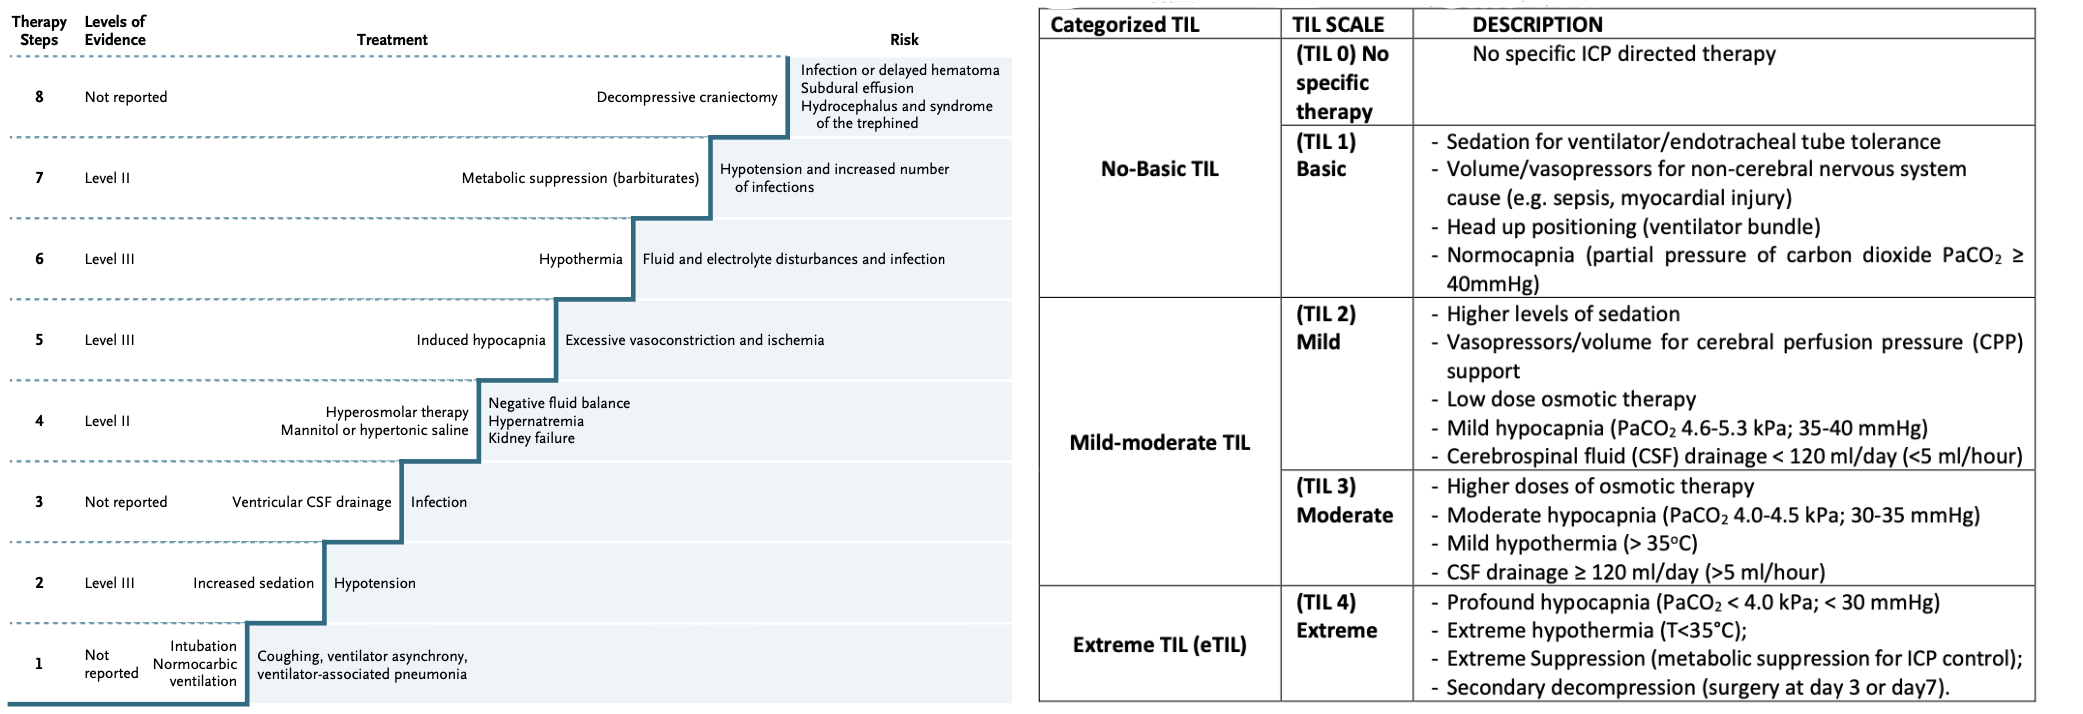
\includegraphics[width=1\textwidth]{pictures/fig4.png}
    \caption{Staircase approach to intracranial hypertension and Therapy Intensity Level scale. Modified from Stocchetti et al.\cite{stocchettiTraumaticIntracranialHypertension2014a} and Robba et al.\cite{robbaTreatmentsIntracranialHypertension2023a}.}
\end{figure}

